%%
%% 2019 07 04 Ph. G. Freimann
%%

\section{Lineare Gleichungen mit Parametern}\index{Gleichungen!lineare mit Parametern}\index{Parameter}
\sectuntertitel{Alle Zahlen sind gleich; nur einige sind gleicher.}
%%\TALSTadBFWA{89}{2.2.2}
%%%%%%%%%%%%%%%%%%%%%%%%%%%%%%%%%%%%%%%%%%%%%%%%%%%%%%%%%%%%%%%%%%%%%%%%%%%%%%%%%
\subsection*{Lernziele}

\begin{itemize}
\item Lineare Gleichungen mit Parametern
\end{itemize}
\TadBMTA{116}{8.2}

Parameter = (wörtlich) «Neben-Maß»

Griechisch $\pi\alpha\rho\alpha$ (para), deutsch: ‚neben‘ und $\mu\epsilon\tau\rho\omega\nu$ (metron) deutsch: ‚Maß‘

\newpage
\subsection{Motivation}
Ein Ladenpreis von CHF 500.- setzt sich zusammen aus ursprünglichem
vom Verkäufer gewünschtem Verkaufspreis $x$ plus der Mehrwertsteuer von 7.7\%.

Wie groß war der ursprüngliche Verkaufspreis $x$?

\TNT{4.8}{
  $x + 7\% \text{von} x = 500$

  $x+\frac{x}{100}\cdot{7.7} = 500$

  $x\cdot{}(1+\frac{7.7}{100})= 500$

  $x\cdot{}(1.077)= 500$

  $x = \frac{500}{1.077} \approx 464.25$
}

Ein Ladenpreis ist CHF 650.-. Darin sind 7.7\% Mehrwertsteuer
enthalten. Was war der Preis vor der Mehrwertsteuer?

\TNT{4.8}{
  $x + 7\% \text{von} x = 650$

  $x+\frac{x}{100}\cdot{7.7} = 650$

  $x\cdot{}(1+\frac{7.7}{100})= 650$

  $x\cdot{}(1.077)= 650$


  $x = \frac{650}{1.077} \approx 603.53$
  
}

Ein Ladenpreis ist CHF $p$. Darin sind 7.7\% Mehrwertsteuer
enthalten. Was war der Preis vorher?

\TNTeop{
  $x + 7\% \text{von} x = p$

  $x+\frac{x}{100}\cdot{7.7} = p$

  $x\cdot{}(1+\frac{7.7}{100})= p$

  $x\cdot{}(1.077)= p$


  $x = \frac{p}{1.077}$
}


\newpage



\TALS{%% TALS Schieberegler im CAS-Rechner

\paragraph{Schieberegler}\index{Schieberegler} Der Taschenrechner \textit{TI-$n$Spire CX
  II-T CAS} kann Terme in der Variablen $x$ parametrisiert
darstellen. Erstellen Sie dazu in einem Dokument eine
\textit{notes}-Page und definieren Sie den Term $terma := a\cdot
x+0.5$. In einem neuen Grafik-Fenster (Page) zum selben Problem
definieren Sie die Funktion $f1(x):=terma$. Damit erscheint die Frage
nach einem Schieberegler, welcher uns den Parameter $a$ verändern
lassen kann.

\bbwCenterGraphic{6cm}{allg/gleichungen/img/LineareFunktionTR_terma.png}
%  \begin{center}
%   \raisebox{-1cm}{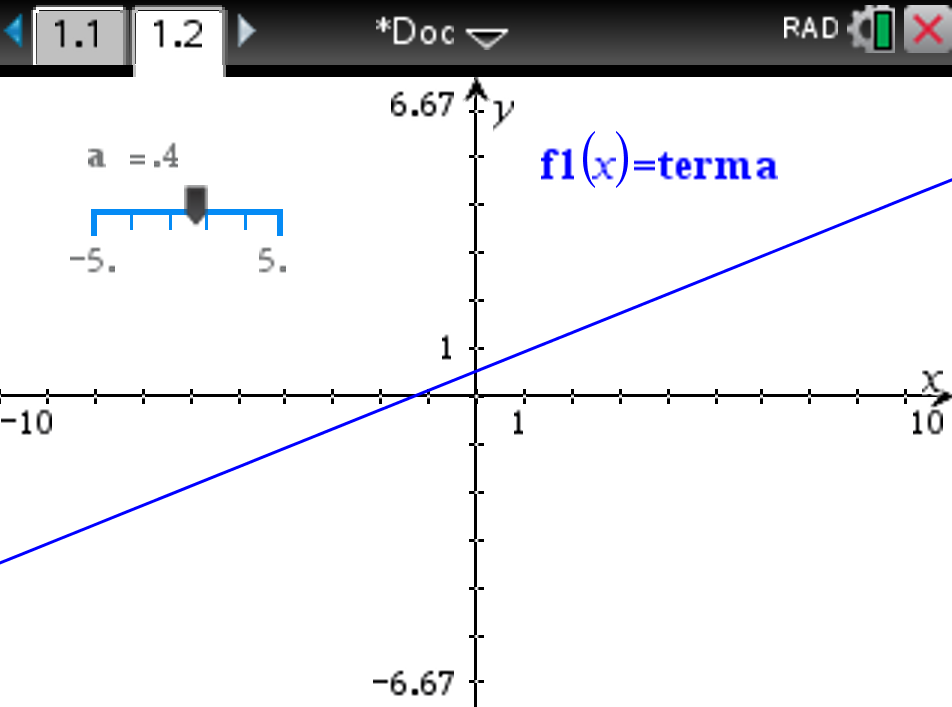
\includegraphics[width=6cm]{img/LineareFunktionTR_terma.png}}
%  \end{center}


\paragraph{Frage 1} Bei welchem Parameter $b$ hat die folgende Gleichung für $x$ die Lösung $1.5$?
$$-2x + b = 0$$

\noTRAINER{$$.....................................$$}
\TRAINER{$$b = 3$$}
Dies lösen wir, indem wir die gesuchte Lösung für $x$ einsetzen und nach $b$ auf"|lösen. Graphisch kann dies auch mit dem CAS-Rechner \textit{gelöst} werden. Definieren Sie «termb := $-2\cdot{}x+b$» und zeichnen Sie den Graphen in einer Graph-Page.
Erstellen Sie einen «Slider»\index{Slider}\index{Schieberegler} für $b$ und ziehen Sie an
diesem \textit{Slider}, bis der Wert der Geraden auf der $x$-Achse den
Wert 1.5 (gesuchte Lösung) angenähert hat.


\paragraph{Frage 2} Bei welchem Parameter $a$ hat die folgende Gleichung für $x$ die Lösung $1.5$?
$$ax-3=0$$

\noTRAINER{$$.....................................$$}
\TRAINER{$$a=2$$}
Dies nähern wir auch mit dem CAS-Rechner an. Definieren Sie den Term
$terma$ neu ($terma := a\cdot{}x-3$) und zeichnen Sie den Graphen in einer Graph-Page.
Ziehen Sie am \textit{Slider}, bis der Wert der Geraden auf der
$x$-Achse dem Wert 1.5 (gesuchte Lösung) genug nahe kommt.
}




%%\TRAINER{Aufg 247 l aus \cite{frommenwiler17alg}}
\subsection{Vorzeigeaufgabe}

\TALS{
  $$\frac{x}{n} + a - \frac{x}{m} + b = mx + c$$
\TNTeop{
  1. Alle $x$ nach links, alle «nicht $x$» nach rechts:

  $$\frac{x}{d}-\frac{x}{m}-mx = c-a-b$$

  2. $x$ ausklamern:

  $$x\left(\frac1n-\frac1m-m\right)=c-a-b$$

  3. durch die Klammer teilen

  $$x=\frac{c-a-b}{\frac1n-\frac1m-m} = (\text{optional}) = \frac{mn(c-a-b)}{m-n-m^2n}$$

}%% END TNT
}%% END TALS

\GESO{
  $$x^2 - \sqrt{2} - c = (b-x)\cdot{}(-\sqrt{5}-x)$$

  \TNTeop{
  Termumformung: $x^2-\sqrt{2} - c = -\sqrt{5}b -bx +x\sqrt{5} + x^2$\\
  beidseitig $-x^2$: $\Rightarrow -\sqrt{2}-c=-\sqrt{5}b-bx+x\sqrt{5}$\\
  Alle $x$ nach links (Rest nach rechts): $\Rightarrow bx-\sqrt{5}x= -\sqrt{5}b+\sqrt{2} + c$\\
  $x$ ausklammern: $\Rightarrow x(b-\sqrt{5})=-\sqrt{5}b+\sqrt{2} + c$\\
  $: (b-\sqrt{5})$ : $\Rightarrow x = \frac{-\sqrt{5}b+\sqrt{2} + c}{b-\sqrt{5}}$\\%%

}%% END TNT
}%% END GESO
\newpage

\subsection*{Aufgaben}
%%\TALS{\aufgabenFarbe{Aufgaben: \cite{frommenwiler17alg} S. 89, Aufg. 246. a) 247. a) c) g) 248. a) d) i) 249.}}

%%\TALS{Textaufgaben: \cite{frommenwiler17alg} S. 89 Aufg. 253}

\AadBMTA{128ff}{ 7. b) c) a) e),
  8. a) d) e) f),
  9. a) b) c) e) f),
  10. a) b)
\TALS{, 11. b) und 12. a) d) e)}
}%% end AadBMTA

\olatLinkGESOKompendium{2.1.3.}{11}{12. bis 16.}

\newpage
